\documentclass{article}
\usepackage{amsmath}
\usepackage{graphicx}
\usepackage{hyperref}

\title{An Exterior Algebra Valued Tutte Function on Linear Matroid Pairs}
\date{March 17, 2025}

\author{Seth Chaiken}
\begin{document}

\maketitle

\begin{abstract}

  Transcription of a 5-min ``Lightning Talk'' presented at
  the workshop
  \href{https://icerm.brown.edu/program/semester_program/sp-s25}{Matroids, Rigidity, and Algebraic Statistics (Mar 17 - 21, 2025)}
  within the
  \href{https://icerm.brown.edu/program/semester_program_workshop/sp-s25-w1}{Geometry of Materials, Packings and Rigid Frameworks
    (Jan 29 - May 2, 2025) program}
  at the \href{https://icerm.brown.edu/}{Institute for Computational and Experimental Research in Mathematics (ICERM), Brown University}.\\

  

  
Let $N$ be a linear representation (i.e, matrix) of a matroid whose
ground set $S$ includes a finite, distinguished subset $P$.  We give
function $L(N)$ that, unlike what we know of other Tutte functions and
work like the Hopf algebra variants of Krajewski, Moffatt and Tanasa,
has values in an \emph{anti-commutative} algebra. Let deletion and
contraction be limited to $e\not\in P$.  Then, the values are in the
exterior algebra generated by $P_\alpha \coprod P_\beta$.  The
construction relies on concrete minor operations to establish
consistent signs of the constituent terms so that, with suitable
accounting for sequential orderings of set elements,
$L(N)=L(N\setminus e)+L(N/e)$ in the exterior algebra. Our
construction is derived from the structure of the equilibrium
equations for linear electrical networks, and of their generalization
to multi-dimensional elastic frameworks.  Further, the construction
does not require orthogonality for the spaces that generalize spaces
of feasible currents and voltages, or of forces and displacements.
Hence $L$ will be defined on equal rank pairs $(N_\alpha, N_\beta)$
(where originally, $N_\alpha=N_\beta=N$).  We take the Tutte
identities those for Welsh and Kayibi's linking polynomial of matroid
pairs. With $N_\alpha\neq N_\beta$, we can derive the digraph
all-minors matrix tree theorem by taking $P$ to be the set of
vertices.  We so get ratio of common basis expansion solutions for
linear electrical and other linear systems with multi-terminal
amplifiers (where a voltage or force at one place is a multiple of
current or displacement at a different place).  To incorporate
resistance ($r_e$), conductance ($g_e$), elasticity coefficient,
etc. parameters, we use parametrized Tutte function theory for which
$L(N)=r_e L(N\setminus e)+ g_e L(N/e)$; the term for common basis $B$
includes $\prod _{e\in B} g_e \prod _{e\not\in B\cup P} r_e$.
\end{abstract}

\pagebreak

\begin{figure}
  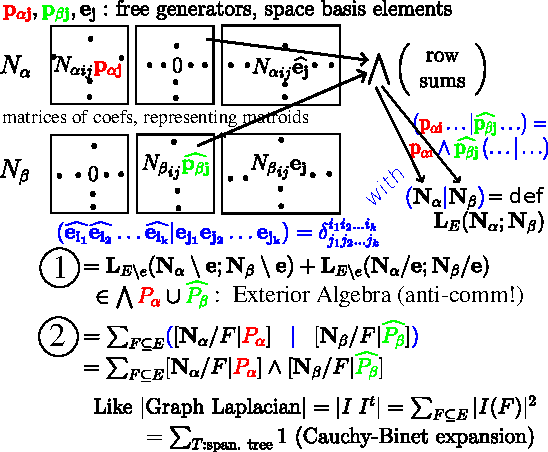
\includegraphics{Brown2025Lightning.pdf}
\end{figure}

   We start with two matrices, $N_\alpha$ and $N_\beta$.  The matroids
    they represent have the $\mathbf{p}$ and $\mathbf{e}$ symbols, each
    exclusively hatted or
    not hatted, for their ground set elements. ...  For now, think of the
    row spaces.

   We make two exterior algebra elements,  boldface
    $\mathbf{N_\alpha}$ and $\mathbf{N_\beta}$ to represent the row spaces.

   We construct function $L$ of those
    $\mathbf{N_\alpha}$ and $\mathbf{N_\beta}$, ... by a bilinear pairing 
    that performs composition ... 
  $\mathbf{N_\alpha} \text{\;\;bar\;\;} \mathbf{N_\beta}$.

   This bilinear operation has exterior algebra,
    not field or commutative ring values. 

 Result 1 is that $L$ obeys Tutte's deletion and contraction identity:  BUT
  only for $e$ type elements, not the $p$'s.  

 There is also a direct sum identity ... $L$ of a direct sum is an exterior product, not
  a commutative ring product.

 We have TO CAREFULLY DEFINE the exterior algebra operations for deletion \&
  contraction \& direct sum so the signs in the $L$--s we combine are consistent.


  As pure, ... or indecomposable anti-symmetric tensors, ... that is, 
  products of vectors, the boldface
  $\mathbf{N}$--s represent linear subspaces of a big space generated
  by matroid ground set elements and their hatted versions.

  So with these designated bases, related to ground sets,
  we get duals of basis vectors.
  The choice of column labels makes hatting consistent with dualizing.
  We'll use duals later.


  $\mathbf{N_\alpha}$ and $\mathbf{N_\beta}$ represent points in the
  Grassmannian, and have Plucker coordinates.
  The Plucker coordinates are the maximal minors of the matrices.
  So, the matroid bases are encoded by which Plucker coordinates are non-zero.


  To construct an extensor from a matrix,
  I multiply each column's boldface symbol with its entries.
  Boldface $\mathbf{N}$ is the exterior product of the row sums.


  Finally $L$ equals the bilinear pairing which expresses an linear endomorphism
  of the exterior algebra generated by the $p$--s.


  I find it interesting that, ... in order to get a Tutte function out
  of this, it seems require two special things.


 We need to make the Tutte function relative.


  That means we to hold some elements back from deletion or contraction,
  ... so they do not all disappear from the algebra where the function value
  will live.


  The distinguished elements we don't delete or contract I like to call PORTS.

%
%  Those port elements in the exterior algebra are vectors, and the hatted
%  ones are covectors, ie., 1-forms or dual vectors.

 In applications, ports relate to variables used to specify inputs
  or parameters, ... like how much you force or electric current you
  put into nodes, ...
  and responses, ... like how the nodes move, or change their voltages.

 But when you use $L$-s value, you can disregard the duality
  status of p elements, ... so 
  you can interchange inputs and responses ANY WAY that the
  matroid of $L$ tells you is feasible and well-posed.  It encodes which
  combinations of variables are independent.
  Electrical engineers like to solve for matrix forms of $L$ and 
  them MULTIPORT LINEAR DEVICE models.

  %The cascade form of two ports has at the first port both the voltage and current for independent, input
  %variables and at the second port, both the voltage and current are response variables. (Not for a
  %lighting talk, just thinking.)


  Two, it seems this exterior algebra Tutte function needs to be constructed on 
  two arguments, labelled $\alpha$ and $\beta$.


  We recover the basis enumerator when the two are equal and $P$ is empty.  It
  is the sum of squared determinants though, not always ones.

 Now for the final step.


  To define the final bilinear pairing function 
  we distinguish 
  four kinds of generators:\\
  vector $\mathbf{e}$'s, vector $\mathbf{p}$'s and
dual vector $\widehat{\mathbf{e}}$ hats and $\widehat{\mathbf{p}}$ hats.  


  It's defined here \emph{WITH} these rules for algebra basis monomials.  Dual vectors
  in the left evaluate on vectors in the right, but reverse that ... and
  they behave like anticommutative coefficients.


  The $\mathbf{N}$--s mix vectors and dual vectors ... they represent linear mappings.
  The hatted and unhatted status of $p$--s and $e$--s are interchanged.
  $\mathbf{N}_\beta$ is like the adjoint of $\mathbf{N_\alpha}$.  So ... the
  bilinear pairing is composition of mappings  ... like matrix multiplication.


  Therefore ... I call this the Cauchy-Binet form.  We get result 2.
  The common independent set expansion here hides many common basis
  expansions.  One of them is the famous matrix tree theorem.

\pagebreak

  I finish with some take-homes and morals, and my name, Seth Chaiken
  of Albany, NY.
  Three punchlines:  One, ports are IM-PORT-ANT.
  Two, let's do matroid recursion on matrices in exterior algebra.
  Three, we find a Tutte function there.
  Thank you!

  \begin{enumerate}
  \item
    Distinguish matroid element ``ports'' associated with 
    electric or elastic system parameter and solution variables of interest.
    (All vars are paired: (voltage, current), (force, displacement), etc.
    One gets a pair of submodels with dual matroids in elementary
    situations; not duals otherwise.)
  \item
    Exterior algebra forms of deletion and contraction of a non-port
    yield a pair of simpler systems.
  \item
    Cancelling non-port elements with a kind of bilinear pairing
    yields the parameter/solution variables of interest relation,
    in the form of an
    \textbf{exterior algebra valued function} of systems,
    that \textbf{is a Tutte function} (when the minor and
    direct sum operations are sign-consistent).
  \end{enumerate}

  With the suitable incidence matrix form, we get the all-minors matrix tree
  theorem; but all the minors are packed into \textbf{one exterior algebra
    object} that is a Tutte function of graphs.

  Seth Chaiken, Assoc. Prof. Emeritus, University at Albany.



\end{document}




\end{document}
